\section{Matrix Operations}
\label{sec:matrix_operations}

Any matrix format used to represent matrices on computers is evaluated with regards to two important benchmarks:
\begin{itemize}
    \item \textbf{Storage}: the storage capacity required to represent the matrix
    \item \textbf{Speed}: the efficiency of calculating certain matrix operations
\end{itemize}

The assessment of the latter might differ depending on which matrix operations are most important for the actual implementation, but usually includes basic building blocks for many other algorithms such as matrix-vector or matrix-matrix multiplication. With regards to linear systems, the performance of Gaussian elimination (i.e. LU factorization) is crucial as well, since it dominates the workload of direct solvers (due to its $\mathcal{O}(n)$ complexity). For iterative solvers, on the other hand, the performance is decided by the speed of the matrix-vector product (at least in the absence of preconditioners).

The details of these operations for the hierarchical formats discussed previously will be detailed in the following sections. Note the discussion within this thesis will be limited to complexity analysis only, but empirical results are available from \cite{spalthoff_pg_hierarchical_2020}.


\section{Matrix-Vector Multiplication}
\label{sec:matrix_vector}

Consider the product resulting from multiplying an  $\mathcal{H}$-matrix $A \in \realx{n}$ with a vector $x$ such that:
\begin{equation}
    Ax = y, \; \; x,y \in \real{}
\end{equation}

\noindent In this case, it is easiest to think of the $\mathcal{H}$-matrix as just a set of general sub-matrices (see e.g. Figure~\hyperref[fig:hodlr]{\ref{fig:hodlr}}) and then it becomes evident that the matrix-vector product is just the result of a summation of operations for each of these matrix blocks. Furthermore, since the actual data is only available in the leaves, only those parts of the cluster tree $\mathcal{T} \in I \times J$ need to be considered. By defining $P = \mathcal{L}(\mathcal{T})$ as the set of leaves of a cluster tree, the following formulation for the matrix-vector product can be obtained (see  \cite{bebendorf_hierarchical_2008}):
\begin{equation}
    y=Ax = \sum_{t \times s \in P}{A_{t,s}x_s}
\end{equation}

\noindent Taking the HODLR storage format as an example, then only diagonal blocks are represented as dense matrices. Hence it follows that the first diagonal block $A_{1,1}$ need to be a leaf-level sub-matrix. Let $A_{1,1}$ be of dimension $10 \times 10$ and let $d = \{1,2,\dots, 10\}$ represent the range. Then the first part of the resulting vector $y_d$ must be given by a sum of the matrix-vector products $A_{t,s}x_s$ where $d$ is part of the range of $s$. This example is illustrated in Figure~\hyperref[fig:matvec]{\ref{fig:matvec}} for easier comprehension, based on the explanation by \cite{ooi_effect_2020}.

\begin{figure}[h]
    \centering
    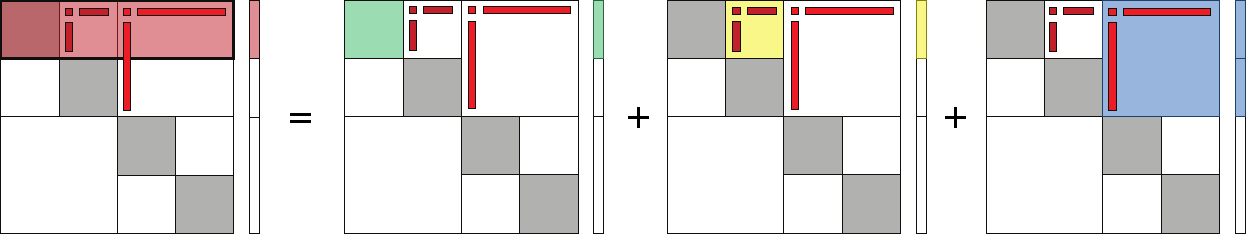
\includegraphics[width=\linewidth]{chapters/4_hierarchical_matrices/figures/matvec.pdf}
    \caption[Hierarchical Matrix-Vector Product]{Example of a HODLR-matrix vector product. The first part of the resulting vector is obtained as a sum of all sub-matrix-vector products that share a row index with the first diagonal leaf-level block (only colored blocks are considered for the multiplication).}
    \label{fig:matvec}
\end{figure}

In case of the first diagonal sub-matrix (and equivalently for every other dense block) the matrix-vector product can be computed just like the standard matrix-vector multiplication. However, if the sub-matrix is a low-rank representation given by $A_{t,s} = UV$, then the result is given by:
\begin{equation}
    A_{t,s}x_s = UVx_s
\end{equation}

\noindent and thus
\begin{equation}
        Vx_s = z_s, \;\; \text{ and }\;\; Uz_s = y_s 
\end{equation}

\noindent Since the workload associated with each low-rank sub-matrix is now bounded in terms of the rank $k$ by at most $2k(|t|+|s|)$ and the dense blocks are rather small (and achieve a similar bound, but with a different constant), matrix-vector multiplication can be performed in $\mathcal{O}(n\;log(n))$ operations (see \cite{bebendorf_hierarchical_2008}), for a balanced cluster tree. In the nested bases case, the amount of work can be further reduced to to the fact that only one multiplication with the basis is necessary. By looking at Figure~\hyperref[fig:hss]{\ref{fig:hss}}, it becomes clear that instead of $Vx_s = z_s$, we know have $TVx_s = z_s$, where $T$ is a small transfer matrix and $V$ corresponds to the shared basis. Thus, by calculating $Vx_s = \Tilde{x}_s$ only once for each row, the computation for the low-rank blocks is reduced to $T\Tilde{x}_s$ and the total work decreases. Analogously, the same argument can be applied to the columns, decreasing the complexity of the matrix-vector product down to $\mathcal{O(n)}$ for $\mathcal{H}^2$-matrices (see \cite{hackbusch_hierarchical_2015} for a complete proof).

\section{Matrix-Matrix Multiplication}
\label{sec:matrix_matrix}

In order to highlight the importance of matrix-matrix multiplication in the context of solving linear systems, a slight extension of the definition is necessary. While a general system of the form $Ax=b$ determines a single solution corresponding to a single right-hand side $b \in \real{}$, many applications actually require solutions to multiple right hand sides $\bm{b}_1, \bm{b}_1, \cdots \bm{b}_m $. Even though the result could be obtained by calculating simple matrix-vector products with different right-hand sides, the computation can be done more efficiently if expressed as matrix-matrix multiplication. Therefore, the system is extended to:
\begin{equation}
    AX=B\text{, } \;\; X=
    \left[
    \begin{array}{c|c|c}
      & & \\
      \bm{x}_1 &\dots & \bm{x}_m \\
      & & \\
    \end{array}
  \right]\text{, } \;\;B=
    \left[
    \begin{array}{c|c|c}
      & & \\
      \bm{b}_1 &\dots & \bm{b}_m \\
      & & \\
    \end{array}
  \right] 
\end{equation}

\noindent In this context, it becomes worthwhile to investigate the performance of matrix-matrix multiplication using the different hierarchical formats. Note that the discussion in this thesis will be limited to the multiplication of two $\mathcal{H}$-matrices, but it is easy to extend the algorithms to a a product of a hierarchical and a dense matrix. By simply dividing the dense matrix according to the same cluster tree a similar partition can be achieved without any admissible blocks. The product can then be obtained by a subset of the operations needed to multiply two $\mathcal{H}$-matrices.

Consider a matrix $A$ built from the cluster tree $\mathcal{T}_{I\times J}$ and a matrix $B$ built from $\mathcal{T}_{J\times K}$. The multiplication of those two will result in a cluster tree $\mathcal{T}_{IJK}$. An exact definition of the resulting cluster tree is given in \cite{bebendorf_hierarchical_2008}, but it should be remarked that simply using $\mathcal{T}_{I\times K}$ is not sufficient, since the bounds on the block-wise rank can not be guaranteed. However, with $\mathcal{T}_{IJK}$ being sufficiently structured, the product is defined for every leaf block $t \times s \in \mathcal{T}_{IJK}$ such that:
\begin{equation}
    (AB)_{t,s} = \sum_{j \in J}A_{t,j}B_{j,s}
\end{equation}

\begin{figure}[h]
    \centering
    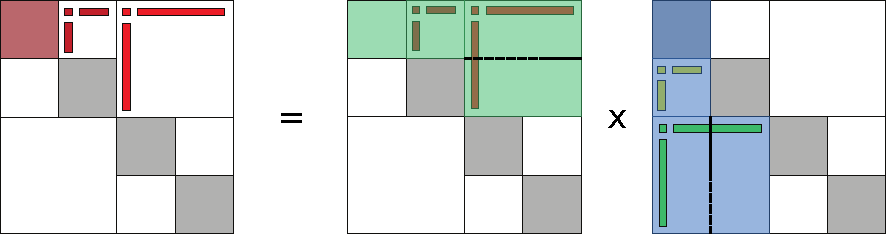
\includegraphics[width=\linewidth]{chapters/4_hierarchical_matrices/figures/matmul.pdf}
    \caption[Hierarchical Matrix-Matrix Product]{Example of a matrix-matrix product in the HODLR format. The first block of the product is obtained as a sum of the blocks within the same row/column (only colored blocks are considered for the multiplication).}
    \label{fig:matmul}
\end{figure}

\noindent This process is illustrated for the first diagonal block of the resulting matrix in Figure~\hyperref[fig:matmul]{\ref{fig:matmul}}. It is easy to see that this requires three kinds of operations:
\begin{itemize}
    \item \textit{Product of two dense matrices}: This corresponds to a normal matrix multiplication and can be calculated via standard formulas (e.g. as provided in \cite{golub_matrix_2013}).
    \item \textit{Product of a dense and a low-rank matrix}: Let $A \in \realx{n}$ be a low-rank matrix with rank $k$ such that $A=UV$ with $U \in \realx[n]{k}$ and $V \in \realx[k]{n}$. The (still low-rank) product with a dense matrix $B \in \realx{n}$ is given by $AB= U\Tilde{V}$, where $\Tilde{V}=VB$.
    \item \textit{Product of two low-rank matrices}: Using the low-rank matrix $A$ from above and similarly defining $B=WZ$ with $W \in \realx[n]{k}$ and $Z \in \realx[k]{n}$, the result can obtained via $AB=\Tilde{U}\Tilde{V}$ with $\Tilde{U}=U(VW)$ and $\Tilde{V}=Z$.
\end{itemize}

\noindent Technically, there is a forth case when none of the involved blocks are leaves of the matrices, which is solved via recursion. Consider the root level ($\ell=0$)of the matrices in Figure~\hyperref[fig:matmul]{\ref{fig:matmul}} and let $\mathcal{H}$ denote a hierarchical and $\mathcal{R}$ a low-rank sub-matrix. The recursion takes the form of:
\begin{equation}
  \left[
    \begin{array}{cc}
       \iter[1]{\mathcal{H}}_{11}& \iter[1]{\mathcal{R}}_{12} \\
      \iter[1]{\mathcal{R}}_{21} & \iter[1]{\mathcal{H}}_{22} \\
    \end{array}
  \right] \cdot 
  \left[
    \begin{array}{cc}
       \iter[1]{\mathcal{H}}_{11}& \iter[1]{\mathcal{R}}_{12} \\
      \iter[1]{\mathcal{R}}_{21} & \iter[1]{\mathcal{H}}_{22} \\
    \end{array}
  \right]=
  \left[
    \begin{array}{cc}
       \iter[1]{\mathcal{H}}_{11} \cdot \iter[1]{\mathcal{H}}_{11} + \iter[1]{\mathcal{R}}_{12} \cdot \iter[1]{\mathcal{R}}_{21}& \iter[1]{\mathcal{H}}_{11} \cdot \iter[1]{\mathcal{R}}_{12}+\iter[1]{\mathcal{R}}_{12} \cdot \iter[1]{\mathcal{H}}_{22} \\
      \iter[1]{\mathcal{R}}_{21} \cdot \iter[1]{\mathcal{H}}_{11} + \iter[1]{\mathcal{H}}_{22} \cdot \iter[1]{\mathcal{R}}_{21}& \iter[1]{\mathcal{R}}_{21} \cdot \iter[1]{\mathcal{R}}_{12}+\iter[1]{\mathcal{H}}_{22} \cdot \iter[1]{\mathcal{H}}_{22} \\
    \end{array}
  \right]
\end{equation}

\noindent The partial product $\iter[1]{\mathcal{H}}_{11} \cdot \iter[1]{\mathcal{H}}_{11}$ is then defined recursively by increasing the level:
\begin{equation}
    \iter[1]{\mathcal{H}}_{11} \cdot \iter[1]{\mathcal{H}}_{11}= 
      \left[
    \begin{array}{cc}
       \iter[2]{\mathcal{H}}_{11}& \iter[2]{\mathcal{R}}_{12} \\
      \iter[2]{\mathcal{R}}_{21} & \iter[2]{\mathcal{H}}_{22} \\
    \end{array}
  \right] \cdot 
  \left[
    \begin{array}{cc}
       \iter[2]{\mathcal{H}}_{11}& \iter[2]{\mathcal{R}}_{12} \\
      \iter[2]{\mathcal{R}}_{21} & \iter[2]{\mathcal{H}}_{22} \\
    \end{array}
  \right]
\end{equation}

\noindent Since a leaf-level block is by definition either dense or low-rank, this recursion is guaranteed to terminate and the matrix-matrix product is obtained. Similar arguments as for the case of the matrix-vector product can be applied (see \cite{hackbusch_hierarchical_2015}, resulting in a complexity of $\mathcal{O}(n \;\log(n)$ for the matrix-matrix multiplication.
Analogously, for $\mathcal{H}^2$-matrices, \cite{borm_h2-matrix_2006} demonstrated that linear complexity can be achieved by optimizing the algorithm.


\section{LU Factorization}
\label{sec:h_lu}
The hierarchical LU factorization can be formulated as a generalization of the blocked right-looking LU algorithm \cite{carratala-saez_exploiting_2019}. However, it is possible to exploit the hierarchical structure of the matrix in order to achieve faster computations. As it is possible to formulate all operations on the leaf-level of the matrix, the only changes necessary in the blocked LU algorithm are due to the hierarchy of the cluster tree (i.e. blocks of varying sizes). The general blocked LU factorization takes the form:
\begin{equation}
    A = 
  \left[
    \begin{array}{cc}
      A_{11}& A_{12} \\
      A_{21} & A_{22} \\
    \end{array}
  \right] = 
  \left[
    \begin{array}{cc}
      L_{11}& 0 \\
      L_{21} & L_{22} \\
    \end{array}
  \right]
  \left[
    \begin{array}{cc}
       U_{11}& U_{12} \\
       0 & U_{22} \\
    \end{array}
  \right]
\end{equation}

\noindent If the $\mathcal{H}$-matrix is constructed from a binary tree, this describes the tasks for each block of the matrix (since it has exactly four children). The following four problems need to be calculated:
\begin{enumerate}
    \item Compute $L_{11}$ and $U_{11}$ using a regular LU decomposition of $A_{11}$.
    \item Compute $U_{12}$ from the update $U_{12} =L_{11}^{-1}A_{12}$.
    \item Compute $L_{21}$ from the update $L_{21} =A_{21}U_{11}^{-1}$.
    \item Compute $L_{22}$ and $U_{22}$ from the LU decomposition of $A_{22}-L_{21}U_{12}$.
\end{enumerate}

\noindent In principle this set of operations is called recursively for each block, starting from the root. Whenever a leaf node is reached, the actual computation will be executed producing a partial result of the decomposition. As a natural conclusion from the $\mathcal{H}$-matrix structure, it follows that an actual factorization is only calculated for diagonal blocks, which are necessarily dense (and thus the  operation is well defined). 2 \& 3 are the only operations executed on low-rank representations, which correspond to simple triangular solves. The only problematic part of the algorithm can be the calculation of the Schur-complement in 4. Because such an update needs to be computed on every level, it can involve the addition of low-rank blocks and the sum of two matrices of rank $k_1$ and $k_2$ may have a rank of $k_1+k_2$. This doubling of the rank is undesirable as it has a negative effect on performance and is usually countered by re-compressing the result in the form of \textit{rounded addition} (see \cite{bebendorf_hierarchical_2008}).

\begin{figure}[h]
    \centering
    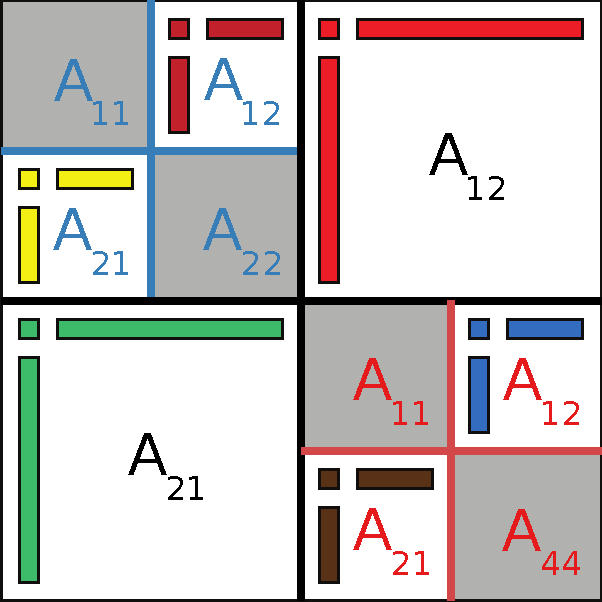
\includegraphics[width=0.6\linewidth]{chapters/4_hierarchical_matrices/figures/hlu.pdf}
    \caption[\texorpdfstring{$\mathcal{H}$}{H}-matrix LU]{Example of the partition used for an LU factorization of a simple HODLR matrix. The splits for different blocks are color-coded.}
    \label{fig:hlu}
\end{figure}

Figure~\hyperref[fig:hlu]{\ref{fig:hlu}} illustrates the structure of the sub-matrices associated with a recursive LU factorization of a $2 \times 2$ partitioning for the HODLR format. The operation starts at the root node and thus tries to factorize the big $A_{11}$  block (in black), which incurs a recursive cal on the splitting denoted in blue. After the recursion finished, blocks $A_{12}$, $A_{21}$ and $A_{22}$ can be updated before the recursion is repeated on the red splitting. It is easy to see, that the actual factorization task is exclusively executed for dense blocks, while low-rank representations are only present in update operations. A full pseudo-code denoting the whole operation is available from \cite{hackbusch_hierarchical_2015}.

The LU decomposition of such a hierarchical matrix can be obtained in $\mathcal{O}(n\;log(n))$, which is considerably faster than the $\mathcal{O}(n^3)$ required by a dense matrix. However, due to the hierarchical structure, efficient parallelization is more difficult to achieve, since the size of the leaves varies. The BLR format removes those implementation obstacles, but as a result, only achieves a performance of order $\mathcal{O}(n^2)$. In recent years, efficient algorithms for the $\mathcal{H}^2$ format have been developed (e.g. \cite{ma_accuracy_2018}), which enable them to calculate such a factorization in linear complexity (i.e. $\mathcal{O}(n)$). 

Unsurprisingly, due to these properties, these formats have been extensively studied as preconditioners for sparse matrices (e.g. \cite{bebendorf_hierarchical_2008}, \cite{xia_fast_2010}, \cite{gatto_preconditioner_2015}). Extending this research to preconditioners for general (dense) linear systems is the purpose of this thesis.